\chapter{RNA Base Pair Steps}
\label{basepairsteps} 
\bibliographystyle{nar}
Before  the turn  of the  century it  was still  not  conceivable that
knowledge-based potentials  could be obtained for  RNA helical regions
due to the  small amount of crystallographic data  available. This was
not the case  for DNA, where enough data for  such potentials has been
available   since   1998  as   shown   by   Olson  and   collaborators
\cite{olson1998}.   As  pointed  out  in  Chapter  2,  the  number  of
high-resolution X-ray  crystal structures of RNA has  increased by two
orders of magnitude, giving us enough information to develop a dimeric
model of double-helical  RNA with 10 unique base-pair  steps formed by
the canonical G$\cdot$C and  A$\cdot$U Watson-Crick pairs. An extended
model with 21  unique dimeric steps can also  be constructed by adding
the wobble G$\cdot$U base-pair  to canonical G$\cdot$C, and A$\cdot$U,
but for the  GU$\cdot$GU (11 cases) and UA$\cdot$UG  (20 cases) dimers
data is still  scarce. An illustration of the  possible unique dimeric
steps which can be formed in RNA as mentioned above is given in Figure
\ref{fig:unique}.

\begin{figure}
\centering
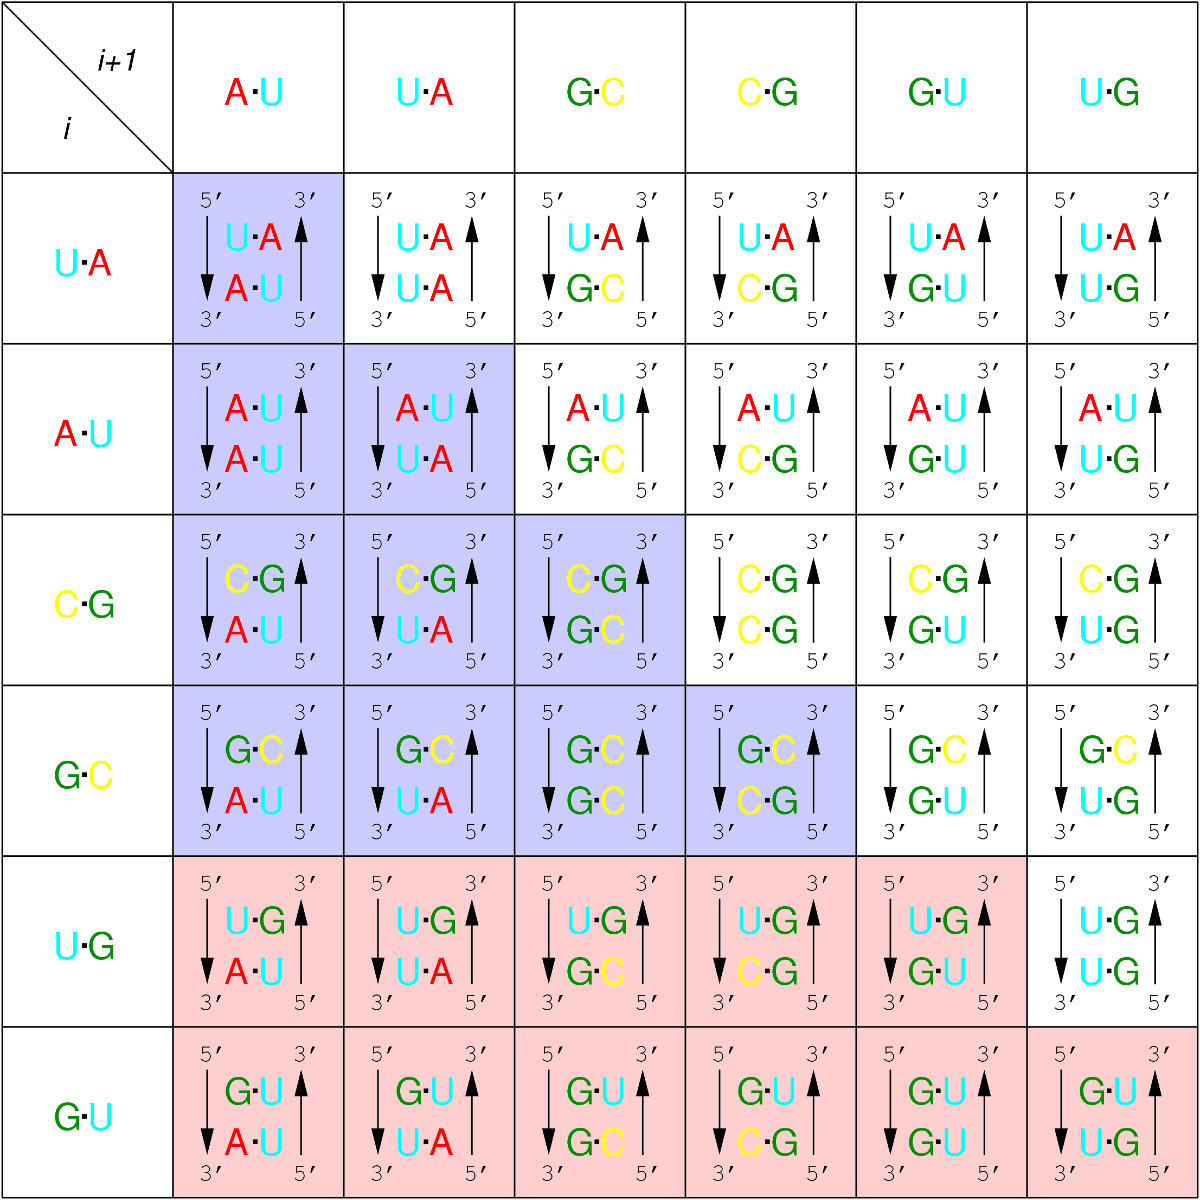
\includegraphics[angle=0, scale=0.4]{Chapter4/unique.png}
\caption{Unique base-pair dimers of RNA formed by canonical G$\cdot$C,
  canonical    A$\cdot$U    Watson-Crick,    and   wobble    G$\cdot$U
  base-pairs.  In purple  boxes the  10 unique  base-pair steps
  formed  by canonical G$\cdot$C  and A$\cdot$U,  and in  beige boxes
  the  additional  11   base-pair  steps  which   result  from
  considering G$\cdot$U  wobble base-pairs as dimer  building block to
  give a total of 21 unique  dimers. The coloring scheme used to color
  the bases is that  used in the NDB, where A is red,  U is cyan, G is
  green, and C is yellow. The first  base-pair in the step in the 5' to
  3' sense is  identified as pair $i$ and the  second is identified by
  $i+1$ as shown in the upper left corner.}
\label{fig:unique}
\end{figure}  

For the  case of the possible  91 unique base-pair steps  which can be
formed from the seven  dominant base-pairing types discussed in Chapter
3,  we see  some tendencies  on the  favoured sequence  preferences as
infered from counts of the available data as will be shown in the next
section. 

The   results  obtained   from  the  analysis   of  RNA knowledge
based dimeric information allow  us to  explore RNA  at  the global
level, that is, as a polymer chain, and compute the persistence length
of some RNA sequences as shown in the last section of this chapter.

\section{Analysis of Base-Pair-Steps}
From  the  dataset  of  base-pairs  described in  Chapter  2  we  also
collected base-pair step information  and focused our attention in the
dimers which are  located in intact helical regions,  those noted as H
in  Figure   \ref{fig:helregxin}.   From  the  data   shown  in  Table
\ref{tab:91steps}  we see that  it's more  common for  a non-canonical
base-pair to  form a  step with a  canonical base-pair partner  than a
non-canonical  one.  The  number of  steps formed  by  a non-canonical
base-pair and a  canonical one is six times higher  than that of steps
formed  by  two non-canonical  pairs.   Some non-canonical  base-pairs
occur exclusively in  the context of a stack  of non-canonicals, e.g.,
GA$_{s}$$\cdot$GA$_{s}$, where two  sheared base-pairs stack together,
or also  on stacks  of a sheared  G$\cdot$A base-pair and  a Hoogsteen
A$\cdot$U  base-pair.  The  majority of  stacks  between non-canonical
base-pairs  is  that of  dimeric  steps  composed  of combinations  of
G$\cdot$U wobble and sheared G$\cdot$A base-pairs. By far the majority
of  dimeric steps  is that  formed by  canonical  G$\cdot$C base-pairs
which make up  more than a third of the whole.  It is also interesting
that more  than half of  this kind of  steps is formed  by GG$\cdot$CC
steps.

The overlap  values between base-pairs are given  in parentheses along
with the  counts of dimeric steps  in intact helical  regions in Table
\ref{tab:91steps}. Looking  at this values  the common trend  seen for
overlaps of DNA base-pairs is respected, i.e., purine-pyrimidine steps
have   the   greatest  overlap   values   and  pyrimidine-purine   the
smallest.  When   the  G$\cdot$U   wobble  base-pair  is   taken  into
consideration the trend remains  true, but the values are considerably
increased,  for example for  the GU$\cdot$GU  dimer. The  other values
which show a large overlap are those of the dimers composed of sheared
G$\cdot$A pairs and those  composed of sheared G$\cdot$A and U$\cdot$U
wobble.  The degree of overlap doesn't necesarily correlate with greater
dimer stabilities as judged from the propensities of observed
dimers,  for example,  wobble U$\cdot$U  pairs prefer  to  stack along
canonical G$\cdot$C pairs with a relatively small overlap.


The  sequence-dependent variation of  base-pair overlap  accompanies
other  subtle changes  in dimeric  structure. For  example,  the twist
angle between  tandem Watson-Crick  G$\cdot$C pairs increases  and the
bending,  via Roll,  becomes  more negative  with  greater base-pair
overlap,  i.e., TwistCG  < TwistGG  < TwistGC  and RollCG  >  RollGG >
RollGC,  where CG,  GG, and  GC denote  the sequence  of bases  on the
leading strand of each dimer. Similar differences occur in DNA, albeit
over  a  much  wider  range  of  conformational  states.  The
sequence-dependent patterns in RNA dimeric structure, illustrated in
Fig. 4 by atomic-level  representations of tandem G$\cdot$C pairs with
the mean step parameters and phosphorus positions found in the current
dataset, are less striking  than the corresponding differences among
the dimeric arrangements of  tandem G$\cdot$U pairs. The non-canonical
pair introduces  noticeable asymmetry in  the sugar-phosphate backbone
at  the  GG$\cdot$UU  step  (Fig.  4).  The  phosphorus  atom  on  the
G-containing strand is displaced by 1.5 \AA and that on the U-containing
strand  by 1.0  \AA relative  to the  corresponding positions  in tandem
G$\cdot$C pairs. Although the phosphorus displacement is smaller and
more  symmetric,  the  twist   angle  differs  appreciably  in  the
G$\cdot$U-containing purine-pyrimidine and pyrimidine-purine dimers
compared to their Watson-Crick counterparts, with the GU$\cdot$GU step
overtwisted  by 15$\circ$  and  the UG$\cdot$UG  step undertwisted  by
-12$\circ$ compared to the GC$\cdot$GC and CG$\cdot$CG steps, respectively. Some
of these  differences reflect the computation  of base-pair parameters
with respect to  a common standard, rather than  a series of reference
frames, one  specific for each  non-canonical pair, that  minimize the
apparent ``discrepancies''.


\begin{sidewaystable}[htbp]
\begin{center}
\begin{tabular}{|c|c|c|c|c|c|c|c|c|c|c|c|c|c|c|}
\hline
C$\cdot$G$_{\text{WC}}$ & G$\cdot$C$_{\text{WC}}$ & U$\cdot$A$_{\text{WC}}$ &
A$\cdot$U$_{\text{WC}}$ & U$\cdot$G$_{\text{w}}$ &
G$\cdot$U$_{\text{w}}$ & A$\cdot$G$_{\text{s}}$ &
G$\cdot$A$_{\text{s}}$ & U$\cdot$A$_{\text{H}}$ &
A$\cdot$U$_{\text{H}}$ & U$\cdot$U$_{\text{w}}$ &
A$\cdot$G$_{\text{WC}}$ & G$\cdot$A$_{\text{WC}}$ & bp$_{i}$/bp$_{i+1}$\\ 
\hline  
604 & 1335 & 747 & 574 & 77 & 192 & 66 & -- & -- & -- & 18 & 4 & 5 & G$\cdot$C$_{\text{WC}}$\\
 & 608 & 511 & 572 & 161 & 252 & 33 & -- & -- & -- & 69 & 20 & 5 & C$\cdot$G$_{\text{WC}}$\\
 &  & 97 & 249 & 20 & 45 & 7 & -- & -- & -- & 2 & -- & 3 & A$\cdot$U$_{\text{WC}}$\\
 &  &  & 126 & 48 & 79 & 6 & -- & -- & -- & 20 & 1 & 14 & U$\cdot$A$_{\text{WC}}$\\
 &  &  &  & 31 & 42 & 32 & 1 & -- & -- & 5 & -- & -- & G$\cdot$U$_{\text{w}}$\\
 &  &  &  &  & 11 & -- & -- & -- & -- & -- & 4 & 7 & U$\cdot$G$_{\text{w}}$\\
 &  &  &  &  &  & -- & 13 & -- & -- & 6 & -- & -- & G$\cdot$A$_{\text{s}}$\\ 
 &  &  &  &  &  &  & 20 & 7 & 2 & -- & -- & -- & A$\cdot$G$_{\text{s}}$\\
 &  &  &  &  &  &  &  & -- & -- & -- & -- & -- & A$\cdot$U$_{\text{H}}$\\
 &  &  &  &  &  &  &  &  & -- & -- & -- & -- & U$\cdot$A$_{\text{H}}$\\
 &  &  &  &  &  &  &  &  &  & 3 & -- & -- & U$\cdot$U$_{\text{w}}$\\
 &  &  &  &  &  &  &  &  &  &  & -- & 1 & G$\cdot$A$_{\text{WC}}$\\
 &  &  &  &  &  &  &  &  &  &  &  & -- & A$\cdot$G$_{\text{WC}}$\\
\hline
\end{tabular}
\caption{Unique base-pair steps parameters counts and overlap values
  in RNA helical regions.}
\label{tab:91steps}
\end{center}
\end{sidewaystable}

  
%Using information derived from a 3.5 Å parsed subset of the
%BPS (Base Pair Structure) database [2] and so-called “inverse harmonic
%analysis” [3], we have derived elastic force constants for the 21
%unique base-pair steps, and are using this simple scoring potential
%model to simulate the fluctuations of RNA helical structures.

\section{RNA Base-Pair-Steps Database and Webframework}
A minimal MySQL database has been  created to store the mean values of
base-step   parameters,   their   standard   deviations,   and   their
corresponding  force constant  matrices. The  purpose of  creating the
database is for  later automatization of the process  of the reduction
of data, that is.


Results from Albany

-Potentials curve plots for steps.



After the work done for the methods paper we extract the force
constant matrices for the 10 unique canonical base-pair steps of RNA
and we use this results to determine the persistence length of RNA
using the sequence-dependent gaussian sampled model (the "realistic"
model) of Olson and collaborators.




\section{Persistence Length of RNA}
A quantity commonly used to  quantify the stiffness of polymers is the
so-called persistence  length $a$. To determine this  quantity for DNA
or RNA,  a variety of  theoretical and experimental techniques  can be
used.  Some  common experimental  techniques to determine  $a$ include
electron   microscopy   (EM),   gel   electrophoresis,   sedimentation
velocities, electrical birefringence,  atomic force microscopy (AFM) ,
magnetic  tweezers,  and small  angle  X-Ray  scattering (SAXS).   For
reviews  of  such  techniques  applied  to the  determination  of  RNA
persistence    length,    we   refer    the    reader   to    Hagerman
\cite{hagerman1997}, Abels  et al.  \cite{abels2005},  and Caliskan et
al.   \cite{caliskan2005}.  We  will compare  our  simulation results,
based on  the "realistic" model  developed by Olson  and collaborators
\cite{olson1995} to describe DNA, with their findings. The "realistic"
model is dependent  on high-resolution crystallographic data.  Initial
studies started with small numbers  of data for the deformabilities of
the  ten unique  base-pair  steps \cite{olson1995}.   A more  complete
picture applied  to the study of DNA  sequence-dependent deformability
became  available   in  1998  \cite{olson1998}.    The  base-pair-step
deformability  data  for  DNA  has  been constantly  refined  as  more
high-resolution DNA and DNA-protein  structures have been added to the
Nucleic Acid Database (NDB) \cite{balasubramanian2009}.  Although such
data has been available for DNA  since 1998, such was not the case for
RNA, until now \cite{olson2009}.

A detailed description of the  ``realistic'' model along with the scheme
of the C++  code developed by Czapla and Zheng to  implement it, and a
brief account of various  definitions of persistence length and models
from which $a$ can be derived are included in Appendix~\ref{appendix4a}

%\section{AMBER: Persistence Length of Base-Pair Step Patterns}
%I guess it needs some input here in order to work on latex compilation.



CHAPTER OUTLINE

- Methods Paper Results / Trends from counts
  - Data culled.
- Step Parameters. Conf Vols, RMSD
- Equipotential Curves

- Webserver
  -table counts
  -table force constants
  -potential curves
  -superimposed structures

- Persistence Length RNA


% Technical pipeline details
%- Collection of base-pair steps data in helical regions.
%  - Yurong's bps database
%  - Yurong's python 3dnaparser
%  - scripts to change signs, assamble unique steps, and do stats.
%  - scripts to cull data
%  - scripts for deformation score
%  - reconstruction and RMSD calculation
%  - scripts for force-constant-matrices


\bibliography{biblio}

